% Created by tikzDevice version 0.12.3.1 on 2022-09-01 15:59:44
% !TEX encoding = UTF-8 Unicode
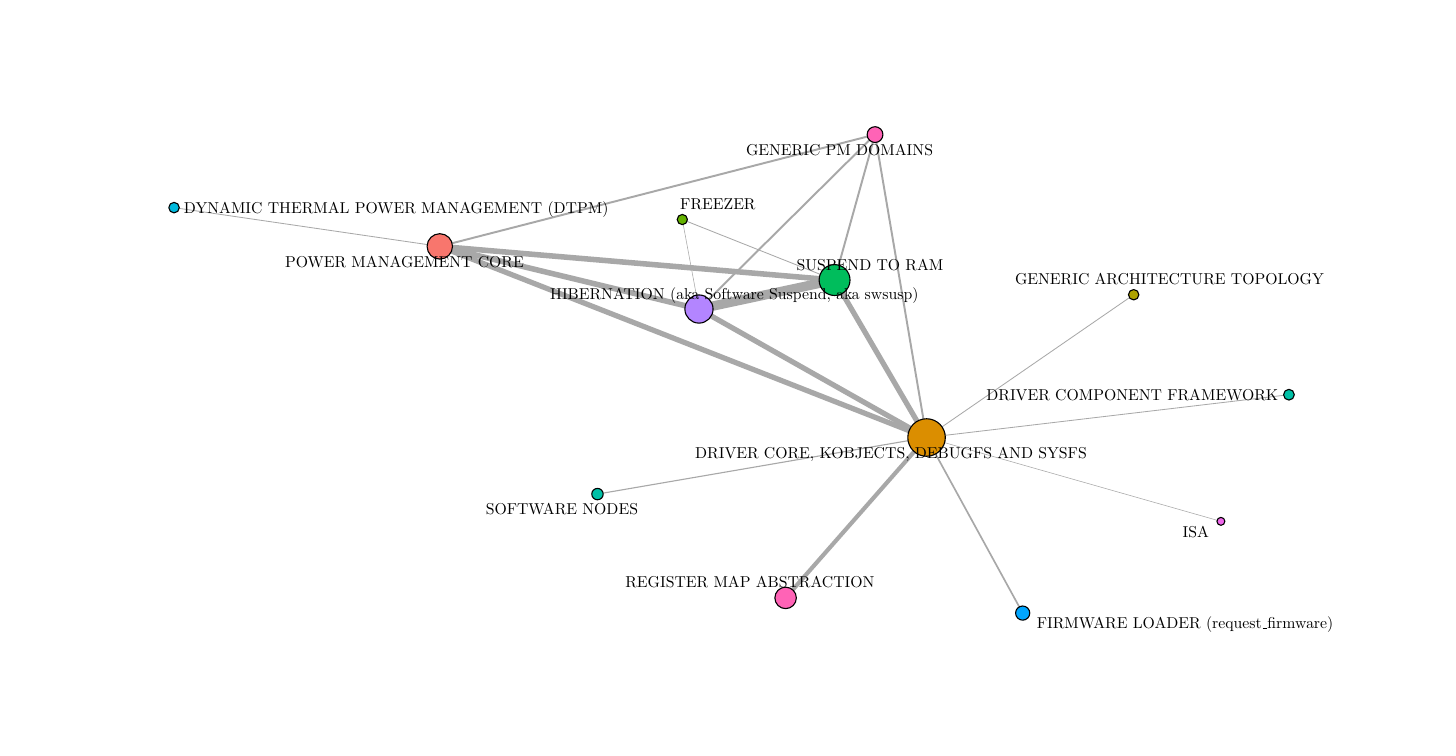
\begin{tikzpicture}[x=1pt,y=1pt]
\definecolor{fillColor}{RGB}{255,255,255}
\path[use as bounding box,fill=fillColor,fill opacity=0.00] (0,0) rectangle (505.89,252.94);
\begin{scope}
\path[clip] (  0.00,  0.00) rectangle (505.89,252.94);
\definecolor{fillColor}{RGB}{255,255,255}

\path[fill=fillColor] (  0.00,  0.00) rectangle (505.89,252.94);
\end{scope}
\begin{scope}
\path[clip] ( 32.75, 32.75) rectangle (475.89,222.94);
\definecolor{drawColor}{gray}{0.66}

\path[draw=drawColor,line width= 0.3pt,line join=round] (455.75,120.31) -- (324.81,104.84);

\path[draw=drawColor,line width= 0.6pt,line join=round] (324.81,104.84) -- (359.54, 41.40);

\path[draw=drawColor,line width= 0.3pt,line join=round] (324.81,104.84) -- (399.65,156.44);

\path[draw=drawColor,line width= 0.7pt,line join=round] (324.81,104.84) -- (306.19,214.30);

\path[draw=drawColor,line width= 1.9pt,line join=round] (324.81,104.84) -- (242.57,151.27);

\path[draw=drawColor,line width= 0.2pt,line join=round] (324.81,104.84) -- (431.17, 74.55);

\path[draw=drawColor,line width= 1.9pt,line join=round] (324.81,104.84) -- (148.92,173.90);

\path[draw=drawColor,line width= 1.5pt,line join=round] (324.81,104.84) -- (273.88, 46.89);

\path[draw=drawColor,line width= 0.4pt,line join=round] (324.81,104.84) -- (205.90, 84.40);

\path[draw=drawColor,line width= 1.9pt,line join=round] (324.81,104.84) -- (291.57,161.74);

\path[draw=drawColor,line width= 0.3pt,line join=round] ( 52.89,187.91) -- (148.92,173.90);

\path[draw=drawColor,line width= 0.2pt,line join=round] (236.55,183.61) -- (242.57,151.27);

\path[draw=drawColor,line width= 0.3pt,line join=round] (236.55,183.61) -- (291.57,161.74);

\path[draw=drawColor,line width= 0.7pt,line join=round] (306.19,214.30) -- (242.57,151.27);

\path[draw=drawColor,line width= 0.7pt,line join=round] (306.19,214.30) -- (148.92,173.90);

\path[draw=drawColor,line width= 0.7pt,line join=round] (306.19,214.30) -- (291.57,161.74);

\path[draw=drawColor,line width= 2.0pt,line join=round] (242.57,151.27) -- (148.92,173.90);

\path[draw=drawColor,line width= 3.4pt,line join=round] (242.57,151.27) -- (291.57,161.74);

\path[draw=drawColor,line width= 2.0pt,line join=round] (148.92,173.90) -- (291.57,161.74);
\definecolor{drawColor}{RGB}{0,0,0}
\definecolor{fillColor}{RGB}{0,193,167}

\path[draw=drawColor,line width= 0.4pt,line join=round,line cap=round,fill=fillColor] (455.75,120.31) circle (  1.94);
\definecolor{fillColor}{RGB}{219,142,0}

\path[draw=drawColor,line width= 0.4pt,line join=round,line cap=round,fill=fillColor] (324.81,104.84) circle (  6.78);
\definecolor{fillColor}{RGB}{0,186,222}

\path[draw=drawColor,line width= 0.4pt,line join=round,line cap=round,fill=fillColor] ( 52.89,187.91) circle (  1.90);
\definecolor{fillColor}{RGB}{0,166,255}

\path[draw=drawColor,line width= 0.4pt,line join=round,line cap=round,fill=fillColor] (359.54, 41.40) circle (  2.56);
\definecolor{fillColor}{RGB}{100,178,0}

\path[draw=drawColor,line width= 0.4pt,line join=round,line cap=round,fill=fillColor] (236.55,183.61) circle (  1.85);
\definecolor{fillColor}{RGB}{174,162,0}

\path[draw=drawColor,line width= 0.4pt,line join=round,line cap=round,fill=fillColor] (399.65,156.44) circle (  1.88);
\definecolor{fillColor}{RGB}{255,99,182}

\path[draw=drawColor,line width= 0.4pt,line join=round,line cap=round,fill=fillColor] (306.19,214.30) circle (  2.85);
\definecolor{fillColor}{RGB}{179,133,255}

\path[draw=drawColor,line width= 0.4pt,line join=round,line cap=round,fill=fillColor] (242.57,151.27) circle (  5.09);
\definecolor{fillColor}{RGB}{239,103,235}

\path[draw=drawColor,line width= 0.4pt,line join=round,line cap=round,fill=fillColor] (431.17, 74.55) circle (  1.43);
\definecolor{fillColor}{RGB}{248,118,109}

\path[draw=drawColor,line width= 0.4pt,line join=round,line cap=round,fill=fillColor] (148.92,173.90) circle (  4.59);
\definecolor{fillColor}{RGB}{255,99,182}

\path[draw=drawColor,line width= 0.4pt,line join=round,line cap=round,fill=fillColor] (273.88, 46.89) circle (  3.88);
\definecolor{fillColor}{RGB}{0,193,167}

\path[draw=drawColor,line width= 0.4pt,line join=round,line cap=round,fill=fillColor] (205.90, 84.40) circle (  2.06);
\definecolor{fillColor}{RGB}{0,189,92}

\path[draw=drawColor,line width= 0.4pt,line join=round,line cap=round,fill=fillColor] (291.57,161.74) circle (  5.58);

\node[text=drawColor,anchor=base,inner sep=0pt, outer sep=0pt, scale=  0.57] at (399.15,118.35) {DRIVER COMPONENT FRAMEWORK};

\node[text=drawColor,anchor=base,inner sep=0pt, outer sep=0pt, scale=  0.57] at (311.96, 97.35) {DRIVER CORE, KOBJECTS, DEBUGFS AND SYSFS};

\node[text=drawColor,anchor=base,inner sep=0pt, outer sep=0pt, scale=  0.57] at (133.16,185.95) {DYNAMIC THERMAL POWER MANAGEMENT (DTPM)};

\node[text=drawColor,anchor=base,inner sep=0pt, outer sep=0pt, scale=  0.57] at (418.23, 35.76) {FIRMWARE LOADER (request{\_{}}firmware)};

\node[text=drawColor,anchor=base,inner sep=0pt, outer sep=0pt, scale=  0.57] at (249.42,187.16) {FREEZER};

\node[text=drawColor,anchor=base,inner sep=0pt, outer sep=0pt, scale=  0.57] at (412.59,160.01) {GENERIC ARCHITECTURE TOPOLOGY};

\node[text=drawColor,anchor=base,inner sep=0pt, outer sep=0pt, scale=  0.57] at (293.36,206.82) {GENERIC PM DOMAINS};

\node[text=drawColor,anchor=base,inner sep=0pt, outer sep=0pt, scale=  0.57] at (255.34,154.82) {HIBERNATION (aka Software Suspend, aka swsusp)};

\node[text=drawColor,anchor=base,inner sep=0pt, outer sep=0pt, scale=  0.57] at (422.08, 68.71) {ISA};

\node[text=drawColor,anchor=base,inner sep=0pt, outer sep=0pt, scale=  0.57] at (136.15,166.44) {POWER MANAGEMENT CORE};

\node[text=drawColor,anchor=base,inner sep=0pt, outer sep=0pt, scale=  0.57] at (260.99, 50.48) {REGISTER MAP ABSTRACTION};

\node[text=drawColor,anchor=base,inner sep=0pt, outer sep=0pt, scale=  0.57] at (193.04, 76.92) {SOFTWARE NODES};

\node[text=drawColor,anchor=base,inner sep=0pt, outer sep=0pt, scale=  0.57] at (304.37,165.30) {SUSPEND TO RAM};
\end{scope}
\end{tikzpicture}
